% =============================================================================
%  What a prime-programmed polymer can read:
%  sieve composition, congruence traps, and arithmetic blindness
%  Paper 3 of the PDTP series.  Draft 1, 1 October 2026.
%  Every number is produced by a script in ../scripts from the CSVs in ../data.
% =============================================================================
\documentclass[reprint,amsmath,amssymb,aps,pre,longbibliography]{revtex4-2}
\usepackage{graphicx}
\usepackage{bm}
\usepackage{amsthm}
\usepackage[colorlinks=true,linkcolor=blue,citecolor=blue,urlcolor=blue]{hyperref}
\graphicspath{{./figures/}}
\newtheorem{theorem}{Theorem}
\newtheorem{corollary}{Corollary}

\begin{document}

\title{What a prime-programmed polymer can read:\\
sieve composition, congruence traps, and arithmetic blindness}

\author{Ruqing Chen}
\email{ruqing@hotmail.com}
\thanks{Archived at \href{https://doi.org/10.5281/zenodo.23094095}{doi:10.5281/zenodo.23094095}.}
\affiliation{GUT Geoservice Inc., Montreal, Quebec, Canada}
\date{\today}

\begin{abstract}
A self-avoiding chain whose bending stiffness follows the gaps of a set of primes (the
prime-driven topological polymer, PDTP) registers the ordering of the prime gaps, but earlier
work showed that this imprint is carried by the smooth prime-number-theorem envelope at the
small-prime end of the chain. Here we ask whether the fold can register anything finer: the
congruence structure that confines twin and Sophie Germain primes to $2\bmod3$ and odd Landau
primes $n^2+1$ to $1\bmod4$, which in localized Bost--Connes systems decides whether the
equilibrium state is unique. We answer in five tests. (i)~A theorem: any order contrast against a
multiset-preserving surrogate is blind to every congruence channel locked by the gap multiset,
which includes all single-class confinements. (ii)~In a prime window at $10^8$, where the
envelope is flat, the Langevin polymer does not distinguish the primes from ten fixed shuffles
at the sequence level ($Z_{\rm seq}=+1.04$, $p=0.33$). (iii)~The exact positional readout of the
ideal chain does not respond to jitter surrogates that null or preserve a single mod-$q$
channel (contrasts $\le0.004$ against a shuffle spread of $0.02$). (iv)~The exact scattering
function does not either; its apparent response is an artefact of the jitter, which changes the
gap multiset, and we show that no jitter pair can avoid this. (v)~What remains is composition.
Against Granville's sieve models drawn with the family's own density envelope and anchor count,
the stiffness composition of every family converges monotonically with sieve depth $z$; the
single-class confinement is the $z=3$ layer of that convergence. The kernel-versus-generator
dichotomy that separates Landau from twin primes in the Bost--Connes setting has no polymer
counterpart: twin primes lie further from their sieve model than Landau primes do, because a
congruence condition affects the polymer in proportion to the ratio of modulus to mean gap. The
polymer reads arithmetic only through the positional envelope and sieve-depth composition.
\end{abstract}

\maketitle

%==============================================================================
\section{Introduction}
%==============================================================================

The prime-driven topological polymer (PDTP) maps the gap between consecutive anchors of an
integer set onto the local bending stiffness of a coarse-grained self-avoiding
chain~\cite{PDTP4}. For the primes, the collapsed chain is measurably less radially sorted than
a chain built from a random permutation of the same gaps, at every size and after complete
relaxation~\cite{PDTP4,Merged}. Two results fix what that imprint is. An exact solution of the
ideal chain shows that any readout carried by chain-scale composition produces the
size-proportional correlation length observed for it, and surrogates that keep only the smooth
prime-number-theorem (PNT) envelope reproduce it~\cite{Merged}. Restricting the readout to bead
subsets shows that the imprint sits at the small-prime end of the chain, where the PNT drift is
steepest~\cite{PDTP4}.

That leaves a sharper question. The primes carry arithmetic structure finer than the envelope:
congruence conditions. Some prime families are confined to a single residue class --- twin and
Sophie Germain primes to $2\bmod3$, odd Landau primes $n^2+1$ to $1\bmod4$ --- and in the
statistical mechanics of localized Bost--Connes systems this confinement matters
decisively~\cite{LBCS,BostConnes}. Confinement to a class that lies in the kernel of a Dirichlet
character (Landau) makes the equilibrium state non-unique at every temperature; confinement to a
class that generates the unit group (twin, Sophie Germain) obstructs nothing~\cite[Ch.~37]{LBCS}.
Does a polymer whose stiffness is programmed by these families register the congruence
structure, and does it distinguish the two kinds of confinement?

We find that it does not, and we show why. Section~\ref{sec:theorem} proves that order contrasts
are blind to congruence channels locked by the gap multiset. Sections~\ref{sec:window}--\ref{sec:sq}
test the remaining routes: a drift-free window, the positional readout, and the scattering
function. Section~\ref{sec:comp} shows that composition is the only channel through which the
congruence structure reaches the fold, measures it against sieve models, and answers the
kernel-versus-generator question. Section~\ref{sec:disc} relates the result to the blindness of
tensorizing invariants in the Bost--Connes setting~\cite[Ch.~4]{LBCS}.

%==============================================================================
\section{Model, families, and surrogates}\label{sec:model}
%==============================================================================

Beads $i=0,\dots,N-1$ are identified with the integers. Given a sorted anchor set $A$, a bead
between consecutive anchors $a<i<a'$ carries the gap $g_i=a'-a$ and an anchor bead carries
$g_i=0$; the stiffness is
\begin{equation}
k_i=\begin{cases}\min\!\left[k_{\rm hinge}e^{\alpha g_i},\,k_{\max}\right], & i\notin A,\\
k_{\rm hinge}, & i\in A,\end{cases}
\label{eq:stiff}
\end{equation}
with $k_{\rm hinge}=0.25$ and $k_{\max}=500$~\cite{PDTP4}. To compare families of very
different density on an equal footing we set $\alpha=0.15\times9.52/\bar g$, so that
$\alpha\bar g$ equals its value for the primes at $N=4\times10^4$.

\emph{Readouts.} The exact ideal chain with bending energy $k_i(1-\cos\theta_i)$ has tangent
correlations $\langle\mathbf t_a\cdot\mathbf t_b\rangle=\prod_{k=a+1}^{b}\mathcal L(k_k)$, with
$\mathcal L$ the Langevin function and $\beta=1$~\cite{PDTP4}. From this we obtain, exactly, the
radius of gyration $R_g^2$; the characteristic ratio $C_N=\langle R_{\rm ee}^2\rangle/(N-1)$; the
mean bond cosine $\langle\mathcal L(k)\rangle$; the curvature energy per bead
$\langle k(1-\mathcal L(k))\rangle$; the positional readout
$\rho_{\rm id}={\rm Spearman}(k_i,\langle|\mathbf r_i-\mathbf r_{\rm cm}|^2\rangle)$, computed in
$O(N)$; and the scattering function in the Gaussian closure,
$S(q)=N^{-1}\sum_{ij}\exp(-q^2\langle R_{ij}^2\rangle/6)$, computed in $O(N^2)$. The Langevin
model of Sec.~\ref{sec:window} adds excluded volume and annealing~\cite{PDTP4,WCA,Ermak}.

\emph{Families.} Anchors below $N$ are the primes; the twin primes (smaller member $p$ with
$p+2$ prime); the Sophie Germain primes ($2p+1$ prime); and the Landau primes $n^2+1$. For
$p>3$ twin and Sophie Germain primes lie in $2\bmod3$, hence in $5\bmod6$, so their gaps lie in
$6\mathbb Z$; odd Landau primes lie in $1\bmod4$, so their gaps lie in
$4\mathbb Z$~\cite[Ch.~37, Lemma~2.1]{LBCS}. Our counts to $2\times10^5$ reproduce the table of
Ref.~\cite[Ch.~37]{LBCS} exactly (2159, 2056 and 63 members).

\emph{Surrogates.} S1 permutes the gaps (exact multiset, order destroyed). The sieve model
$S_7$-G$(z)$ is Granville's refinement of Cram\'er's model~\cite{Cramer,Granville}, adapted to
each family: its candidates are the integers that pass the family's own sieve conditions at depth
$z$ (primes: $n$; twin: $n$ and $n+2$; Sophie Germain: $n$ and $2n+1$; Landau: $n^2+1$), each
coprime to $\prod_{p\le z}p$ or itself a prime $\le z$. We draw it bin by bin: bins hold 20
consecutive family members and each bin receives the family's own count. This holds the anchor
count and the smooth density envelope fixed, so that $S_7$-G$(z)$ differs from the family only
in arithmetic, and $z$ orders the arms by arithmetic depth. $z=1$ imposes no sieve; for Landau it
keeps the polynomial support $n^2+1$. The Poisson arm draws from all integers with the same
binning. Finally, the jitter pair of Sec.~\ref{sec:rho} shifts every interior anchor by a random
integer and re-sorts, keeping both end anchors fixed and every shifted anchor between them: the
\emph{kill} arm by $\varepsilon\sim\mathrm U\{0,\dots,q-1\}-\lfloor(q-1)/2\rfloor$, which nulls
every Bragg channel $a/q'$ with $q'\mid q$; the \emph{keep} arm by $q\,b$, $b\sim\mathrm U\{0,1\}$,
which preserves them exactly. Section~\ref{sec:sq} adds a variance-matched keep arm.

%==============================================================================
\section{Order blindness to locked channels}\label{sec:theorem}
%==============================================================================

Write the Bragg amplitude of an anchor set at rational frequency $a/q$ as
$B_{a/q}(A)=|A|^{-1}\sum_{x\in A}e^{2\pi i xa/q}$.

\begin{theorem}[Order blindness]\label{thm:blind}
Let all gaps of $A$ lie in $q\mathbb Z$. Then every multiset-preserving reordering $A'$ of the gaps
with the same first anchor satisfies $|B_{a/q'}(A')|=|B_{a/q'}(A)|=1$ for every $q'\mid q$. In
particular, for any readout $\mathcal R$, the contrast between the true family and a
multiset-preserving surrogate class carries no information about the confinement of the family
to one residue class modulo $q$.
\end{theorem}
\begin{proof}
If every gap is a multiple of $q$, every anchor is congruent to the first anchor modulo $q$, for
any order of the gaps. All terms of $B_{a/q'}$ then have the same phase, and the amplitude has
modulus one in both arms.
\end{proof}

\noindent The fixed first anchor is not needed. If a reordering starts from a different anchor
$c$, every anchor is congruent to $c$ modulo $q$, and the amplitude is the overall phase
$e^{2\pi i ca/q'}$, of modulus one. The statement is therefore invariant under any translation
of the window.

\begin{corollary}
For twin and Sophie Germain primes ($q=6$) and for odd Landau primes ($q=4$) the single-class
confinement is invisible to every True-versus-shuffle contrast, including all those of
Refs.~\cite{PDTP4,Merged}.
\end{corollary}

The theorem closes the route that earlier surrogate hierarchies relied on: ordering contrasts can
detect structure in how the gaps are arranged, but a confinement to one class is not an
arrangement. It is a property of the gap values, that is, of composition. The remaining sections
test whether the fold registers congruence structure by any other route.

%==============================================================================
\section{A drift-free window}\label{sec:window}
%==============================================================================

If the ordering imprint of the primes contained anything beyond the PNT envelope, it would survive
where the envelope is flat. In the window $[10^8,10^8+10^4)$ the relative change of $\ln i$ across
the chain is $5\times10^{-6}$. We folded its 551 primes with the Langevin model of
Ref.~\cite{PDTP4} (5000 annealing steps; $\alpha$ rescaled to $0.0806$ to keep the stiffness
contrast of the origin chain) and compared them with shuffles at the sequence level: $K=10$ fixed
shuffle sequences with $m=5$ trajectories each (Table~\ref{tab:window},
Fig.~\ref{fig:window}).

\begin{table}[t]
\caption{Drift-free window $[10^8,10^8+10^4)$, Langevin model. Upper block: arms with a fresh
surrogate sequence per trajectory, $n=40$, mean $\pm$ s.e.m. Lower block: one-way analysis of the
fixed-shuffle class and the sequence-level contrast with the true chain.}
\label{tab:window}
\footnotesize
\begin{ruledtabular}
\begin{tabular}{lcc}
arm & $\rho$ & Welch $p$ vs true \\ \hline
true primes & $+0.2429\pm0.0075$ & --- \\
S1 (fresh) & $+0.2108\pm0.0076$ & $0.004$ \\
S7 (IAAFT)~\cite{SchreiberSchmitz} & $+0.2196\pm0.0080$ & $0.038$ \\
$S_7$-G$(5)$ & $+0.2450\pm0.0097$ & $0.87$ \\
$S_7$-G$(5)$ shuffled, run-paired & $+0.2398\pm0.0087$ & $0.79$ \\ \hline
fixed S1 class, $K\times m$ & \multicolumn{2}{c}{$10\times5$} \\
$\hat\mu$, $\hat\sigma_{\rm seq}$, $\hat\sigma_{\rm th}$ & \multicolumn{2}{c}{$+0.2241$, $0.0143$, $0.0477$} \\
true $-\hat\mu$, $Z_{\rm seq}$ ($p$) & \multicolumn{2}{c}{$+0.019$, $+1.04$ ($0.33$)} \\
sequence means above true & \multicolumn{2}{c}{3 of 10} \\
\end{tabular}
\end{ruledtabular}
\end{table}

\begin{figure}[t]
\centering
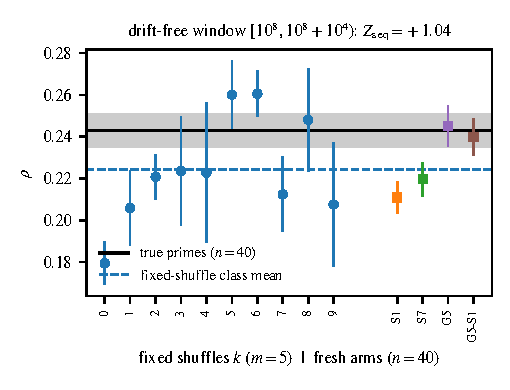
\includegraphics[width=\linewidth]{fig1_m_window.pdf}
\caption{Drift-free window. Dots: the ten fixed shuffle sequences (mean $\pm$ s.e.m.\ of five
trajectories each); dashed line: their class mean. Black line and band: the true primes. Squares:
fresh-sequence arms (S1, IAAFT, sieve model $z=5$ and its run-paired shuffle).}
\label{fig:window}
\end{figure}

The naive Welch test against fresh shuffles gives $p=0.004$. It is anti-conservative. The
between-sequence standard deviation of the shuffle class, $\hat\sigma_{\rm seq}=0.014$, is of
the order of the effect itself, and it enters the variance of the contrast without shrinking with
the number of trajectories~\cite{PDTP4}. At the sequence level the true chain is an ordinary
member of the shuffle class: three of the ten fixed shuffles fold more sorted than the primes,
and $Z_{\rm seq}=+1.04$. Inside the sieve model the ordering effect is absent as well
($+0.005$, $p=0.68$, run-paired). The exact ideal readout agrees ($z=+0.9$ in the window,
Ref.~\cite{PDTP4}). Where the envelope is flat, the fold does not distinguish the primes from
their shuffles.

%==============================================================================
\section{The positional readout and single channels}\label{sec:rho}
%==============================================================================

The theorem does not exclude a response to channels that the multiset does not lock, such as the
mod-6 doublet of the primes, the strongest Bragg line after parity
($|B_{a/6}|^2=0.25$)~\cite{Torquato2018}. We test it with the jitter pair at $N=4\times10^4$
(Table~\ref{tab:rho}).

\begin{table}[t]
\caption{Exact positional readout $\rho_{\rm id}$ at $N=4\times10^4$, 40 realizations per arm.
$n$: anchors (SG: Sophie Germain). $z$: true family against the S1 ensemble. $\Delta$: mean change of $\rho_{\rm id}$ under the
kill and keep jitter arms relative to the true family.}
\label{tab:rho}
\footnotesize
\setlength{\tabcolsep}{3pt}
\begin{ruledtabular}
\begin{tabular}{lrrrrrr}
 & & & \multicolumn{2}{c}{$q=3$} & \multicolumn{2}{c}{$q=6$}\\
family & $n$ & $z$ & $\Delta_{\rm kill}$ & $\Delta_{\rm keep}$ & $\Delta_{\rm kill}$ & $\Delta_{\rm keep}$\\ \hline
primes & 4203 & $-2.4$ & $+0.0007$ & $+0.0016$ & $+0.0015$ & $+0.0037$\\
twin & 591 & $0.0$ & $+0.0001$ & $-0.0005$ & $+0.0004$ & $+0.0001$\\
SG & 565 & $0.0$ & $+0.0001$ & $+0.0004$ & $0.0000$ & $+0.0013$\\
Landau & 34 & $-1.4$ & $0.0000$ & $-0.0001$ & $0.0000$ & $+0.0001$\\
\end{tabular}
\end{ruledtabular}
\end{table}

Every jitter contrast is below $0.004$, against a shuffle standard deviation of about $0.02$, and
the kill and keep arms --- which differ precisely in whether the channel survives --- move the
readout by the same small amount. Only the primes separate from their shuffles at all ($z=-2.4$),
and that separation is the envelope effect of Refs.~\cite{PDTP4,Merged}. The positional readout
does not see single congruence channels.

%==============================================================================
\section{The scattering function, and why jitter cannot isolate a channel}\label{sec:sq}
%==============================================================================

The scattering function is the natural candidate for a channel-sensitive readout: a periodic
modulation of the stiffness should produce a structure in $S(q)$. Figure~\ref{fig:sq} shows the
exact $S(q)$ of the ideal chain for the primes ($N=6000$) and the twin primes ($N=12000$),
relative to the shuffle ensemble.

\begin{figure*}[t]
\centering
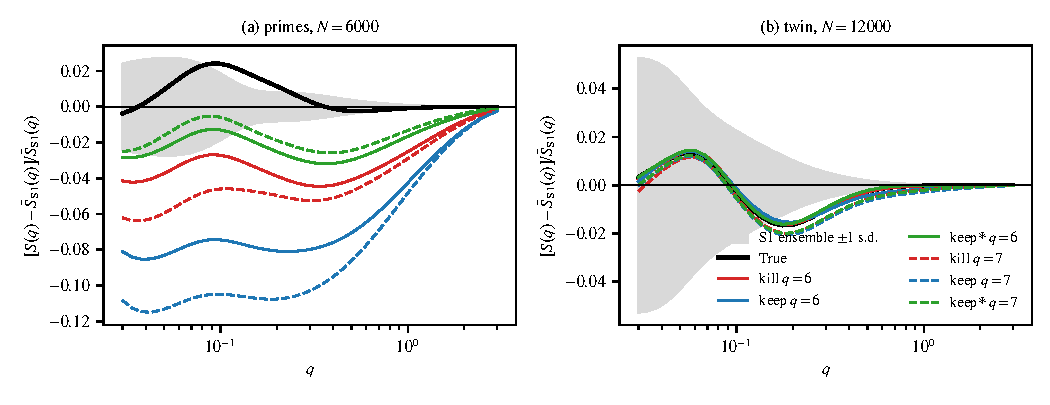
\includegraphics[width=\linewidth]{fig2_sq_channel.pdf}
\caption{Exact $S(q)$ of the ideal chain relative to the shuffle ensemble (grey band: $\pm1$ s.d.).
Black: true family. Red, blue, green: kill, keep and variance-matched keep (keep$^*$) jitter arms,
at the heavy modulus $q=6$ (solid) and the light modulus $q=7$ (dashed).}
\label{fig:sq}
\end{figure*}

The true family lies inside the shuffle band: its largest deviation is $2.4\%$ for the primes and
$1.7\%$ for the twin primes, at most $2.0$ standard deviations of the shuffle ensemble. The jitter
arms for the primes lie far outside the band, but their displacement does not track the channel.
The heavy modulus $q=6$, whose divisor channels carry Bragg weight $W_3+W_6=1$, moves $S(q)$ no
more than the light modulus $q=7$, with $W_7=1/6$~\cite{LBCS}: the mean shift is $-3.0\%$ (kill)
and $-6.1\%$ (keep) at $q=6$ against $-4.1\%$ and $-8.0\%$ at $q=7$. The size of the shift
follows the jitter design instead. The variance-matched keep$^*$ arm, which perturbs the gap
multiset least (Table~\ref{tab:audit}), shifts $S(q)$ least ($-1.9\%$ and $-1.5\%$), and the
three designs rank exactly as their changes of gap variance do. The double difference
$[\Delta(6)-\Delta(7)]$, which removes the common mechanical perturbation, is at most $2.2\%$,
$3.1\%$ and $0.8\%$ for the three designs on the primes, with the light modulus contributing
the larger shift, and at most $0.6\%$ on the twin primes, whose jitter arms all stay within
$2.1\%$ of the shuffle ensemble.

The reason is that the jitter changes the gap multiset, and the polymer is sensitive to
composition. Table~\ref{tab:audit} audits the three jitter designs on the primes. The keep arm of
the original design moves anchors by $q$ or $0$, with displacement variance $q^2/4$, three times
the kill arm's $(q^2-1)/12$, and doubles the change in gap variance. Matching the displacement
variance (keep$^*$: $\pm q$ with probability $(q^2-1)/24q^2$ each) does not cure it. The matched
arm moves few anchors far while the kill arm moves all anchors a little, and their gap multisets
still differ by a factor of four in KS distance. This is not a defect of a particular design. By
Theorem~\ref{thm:blind}, any construction that changes a congruence channel must change gap
values. A value change that acts only through residues modulo $q$ has its displacements on
$q\mathbb Z$ in one arm and spread over $\mathbb Z/q\mathbb Z$ in the other, so the two arms cannot have
the same gap statistics.

\begin{table}[t]
\caption{Jitter audit, primes, $N=4\times10^4$, 20 realizations: KS distance of the perturbed
gap multiset to the true one, relative change of the gap variance, and Bragg power at $a/q$
(true: $0.249$ at $q=6$, $0.028$ at $q=7$).}
\label{tab:audit}
\begin{ruledtabular}
\begin{tabular}{llccc}
$q$ & arm & KS & $|\Delta{\rm Var}\,g|/{\rm Var}\,g$ & Bragg $a/q$\\ \hline
6 & kill & 0.083 & 0.071 & $2.0\times10^{-4}$\\
6 & keep & 0.071 & 0.159 & 0.25\\
6 & keep$^*$ & 0.021 & 0.050 & 0.25\\
7 & kill & 0.086 & 0.094 & $2.4\times10^{-4}$\\
7 & keep & 0.107 & 0.155 & 0.028\\
7 & keep$^*$ & 0.032 & 0.048 & 0.028\\
\end{tabular}
\end{ruledtabular}
\end{table}

%==============================================================================
\section{Composition against sieve models}\label{sec:comp}
%==============================================================================

Sections~\ref{sec:theorem}--\ref{sec:sq} together show that congruence content cannot be varied
in a multiset-preserving design, and cannot be varied without varying composition in a
value-perturbing one. A test of congruence structure in the polymer must therefore vary both
together, along a family of anchor sets defined arithmetically and otherwise matched. The binned
sieve models $S_7$-G$(z)$ are such a family. Table~\ref{tab:comp} and Fig.~\ref{fig:comp} compare
each family with them at $N=10^6$.

\begin{table*}[t]
\caption{Prime families against their sieve models at $N=10^6$, 40 realizations per arm, exact
ideal chain. KS: excess Kolmogorov--Smirnov distance between the bead-stiffness distributions of
the true family and the arm (the distance between two realizations of the arm subtracted).
$z(\cdot)$: true family against the arm, in units of the arm's standard deviation, for the mean
bond cosine, the radius of gyration and the positional readout. $f_6$, $f_4$: fractions of
gaps divisible by 6 and by 4 (true values in the first row of each block).}
\label{tab:comp}
\begin{ruledtabular}
\begin{tabular}{llrrrrrr}
family (anchors) & arm & KS & $z(\langle\mathcal L\rangle)$ & $z(R_g^2)$ & $z(\rho_{\rm id})$ & $f_6$ & $f_4$\\ \hline
primes (78\,498) & true & --- & --- & --- & --- & 0.418 & 0.425\\
 & S1 & 0.000 & $-0.9$ & $+6.9$ & $-7.4$ & 0.418 & 0.425\\
 & $z=1$ & 0.093 & $-63.4$ & $-27.0$ & $-0.8$ & 0.135 & 0.221\\
 & $z=3$ & 0.037 & $-24.6$ & $-14.2$ & $-0.5$ & 0.434 & 0.443\\
 & $z=5$ & 0.020 & $-13.9$ & $-13.7$ & $0.0$ & 0.426 & 0.430\\
 & $z=7$ & 0.013 & $-7.9$ & $-8.2$ & $-0.1$ & 0.422 & 0.428\\ \hline
twin (8\,169) & true & --- & --- & --- & --- & 1.000 & 0.473\\
 & $z=1$ & 0.053 & $-11.9$ & $-3.9$ & $-0.3$ & 0.164 & 0.247\\
 & $z=3$ & 0.039 & $-10.7$ & $-4.3$ & $-0.3$ & 1.000 & 0.487\\
 & $z=5$ & 0.028 & $-6.6$ & $-3.0$ & $0.0$ & 1.000 & 0.482\\
 & $z=7$ & 0.014 & $-6.3$ & $-2.8$ & $-0.4$ & 1.000 & 0.473\\ \hline
Sophie Germain (7\,746) & true & --- & --- & --- & --- & 1.000 & 0.477\\
 & $z=1$ & 0.041 & $-9.8$ & $-3.6$ & $-0.1$ & 0.164 & 0.247\\
 & $z=3$ & 0.029 & $-8.9$ & $-2.8$ & $-0.3$ & 1.000 & 0.486\\
 & $z=5$ & 0.017 & $-6.3$ & $-2.5$ & $+0.1$ & 1.000 & 0.482\\
 & $z=7$ & 0.008 & $-3.0$ & $-1.6$ & $-0.1$ & 1.000 & 0.476\\ \hline
Landau (112) & true & --- & --- & --- & --- & 0.396 & 0.991\\
 & $z=1$ & $<0$ & $-1.8$ & $+0.8$ & $-0.1$ & 0.228 & 0.463\\
 & $z=3$ & $<0$ & $-1.3$ & $+1.5$ & $-0.1$ & 0.501 & 0.996\\
 & $z=7$ & 0.004 & $0.0$ & $+1.8$ & $0.0$ & 0.492 & 0.995\\
\end{tabular}
\end{ruledtabular}
\end{table*}

\begin{figure*}[t]
\centering
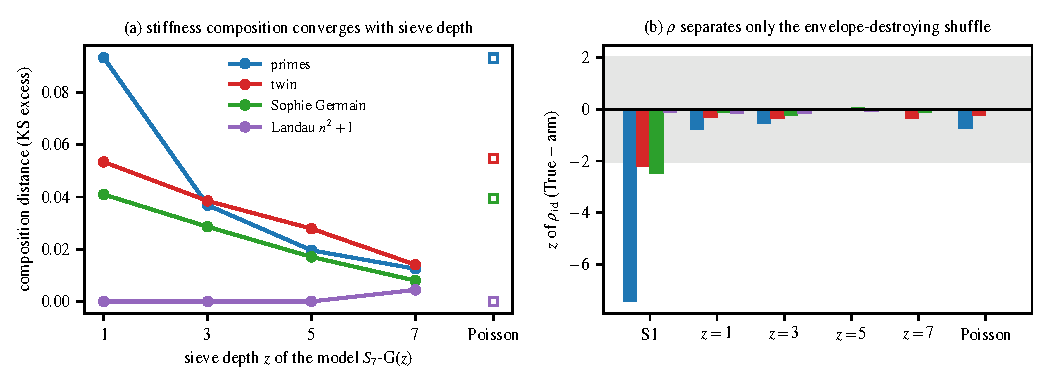
\includegraphics[width=\linewidth]{fig3_composition.pdf}
\caption{(a)~Composition distance of each family to its sieve model as a function of the sieve
depth $z$ (open squares: Poisson; negative values, i.e. closer than two realizations of the arm, are drawn at zero). (b)~$z$-score of the positional readout $\rho_{\rm id}$ of the
true family against each arm; grey band $|z|<2$. Only the S1 shuffle, which destroys the density
envelope, separates the primes.}
\label{fig:comp}
\end{figure*}

\emph{Composition converges with sieve depth.} For every family the composition distance falls
monotonically as $z$ grows. The coarse readouts follow it: the mean bond cosine of the primes
moves from $z=-63$ against the unsieved model to $-8$ at $z=7$. Convergence is not complete at
$z=7$ for the primes, since their sieve continues to $\sqrt N$; the polymer registers sieve depth
well beyond the first few primes.

\emph{The congruence trap is the $z=3$ layer.} For twin and Sophie Germain primes the gaps
divisible by 6 rise from $16\%$ in the unsieved model to $100\%$ at $z=3$, exactly as in the
true family. The remaining composition distance then decreases gradually through $z=5$ and $7$.
There is no discontinuity at the trap. The single-class confinement is one layer of sieve
composition among many, not a separate kind of structure.

\emph{The positional readout is blind to all of it.} No sieve model is separated from its family
by $\rho_{\rm id}$ ($|z|\le0.8$), while the S1 shuffle, which keeps composition and destroys the
envelope, separates the primes at $z=-7.4$. This is the third independent confirmation that
$\rho$ reads the positional envelope~\cite{PDTP4,Merged}.

\emph{Kernel versus generator.} In the Bost--Connes setting, Landau primes are permanently
obstructed and twin primes are not~\cite[Ch.~37, Thm.~2.2]{LBCS}. In the polymer the order is
reversed, and the kernel condition plays no role. Twin primes stay distinguishable from their
sieve model up to $z=7$ ($z(\langle\mathcal L\rangle)=-6.3$). Landau primes are indistinguishable
from every arm on every physical readout ($|z|\le2.8$), even the unsieved arm, in which only
$46\%$ of the gaps are multiples of 4. The $4\mathbb Z$ property of Landau gaps is itself a
consequence of parity. Every odd Landau prime has $n$ even, so the gap between any two of them is
$(n_2^2+1)-(n_1^2+1)=(n_2-n_1)(n_2+n_1)$, a product of two even numbers, hence in $4\mathbb Z$. More to the point, a congruence
condition modulo $q$ alters the stiffness composition in proportion to $q/\bar g$. It is $0.05$
for twin primes at $N=10^6$ ($q=6$, $\bar g=122$) and $5\times10^{-4}$ for Landau primes ($q=4$,
$\bar g=8759$). The Landau family has only 112 anchors at this size, so its null result has low
power. The ratio $q/\bar g$, however, makes the same prediction at any size.

%==============================================================================
\section{Discussion}\label{sec:disc}
%==============================================================================

The five tests leave one picture. A prime-programmed polymer registers arithmetic through two
channels only. The first is the positional envelope: how the stiffness composition changes along
the chain, which for the primes from the origin is the PNT drift~\cite{PDTP4,Merged}. The second
is the composition of the gap multiset, which converges to that of the family as the sieve
depth of a model grows. Congruence structure reaches the polymer only as part of the second
channel, in proportion to the modulus over the mean gap, and only when the comparison changes
composition. No readout we tested responds to the arrangement of residues: not the rank
statistic of the collapsed globule, not the positional readout, not the scattering function.

The pattern has a structural parallel in the localized Bost--Connes systems, where the arithmetic
of a set of primes lives in the measure class of the equilibrium states and every invariant that
tensorizes over the local factors --- $K$-theory, factor type, spectral distance, dynamical
entropy --- is blind to it~\cite[Ch.~4]{LBCS}. The polymer readouts share the relevant feature:
each is a sum, or a rank statistic of a sum, of local contributions, and the only nonlocal input
is a bead's position along the chain. The difference in kind is worth stating. The polymer's
equilibrium is a Gibbs measure on conformation space, for one fixed sequence, and its observables
are integrals of local functions of the conformation. The KMS measures of the Bost--Connes
systems live on a different space, the arithmetic space on which the Hecke semigroup acts, and
it is the measure class of those measures that carries the arithmetic. The polymer has no access
to that space or to the operator-algebraic structure built on it. Its readouts are expectations of
local, additive quantities, the counterpart of the tensorizing invariants rather than of the
measure class. We state the parallel as an analogy and not as a theorem.
The polymer is not a C$^*$-dynamical system, and the kernel condition that decides uniqueness of
the KMS state is a statement about the divergence of character-weighted sums over the family,
for which the polymer has no counterpart. The experiment shows that it has none in practice
either: the ordering of the families by distance from their sieve models is the opposite of
their ordering by obstruction.

The same conclusion bears on the surrogate methodology of the series. A surrogate test of a
physical readout can attribute an effect to ordering only through a multiset-preserving null,
and Theorem~\ref{thm:blind} shows that such a null is silent on single-class confinements. A test
of congruence structure must change composition, and then a controlled family of composition
changes, ordered by arithmetic depth, is required. The binned sieve models provide one. We
expect the same design to be useful for any physical probe of number-theoretic
sequences~\cite{Odijk,KhokhlovKhalatur}.

\emph{Limitations.} Most of the results are exact statements about the ideal chain. Excluded volume
and collapse enter only through the drift-free window, which uses one size and one protocol. The
Landau family is small at accessible sizes. Composition is summarized by a KS distance between
stiffness distributions and by a handful of coarse readouts; finer composition statistics might
order the families differently. The sieve models are drawn with a fixed bin width of 20 members,
so envelope structure on shorter scales is not controlled. Contact-network invariants of the
collapsed globule are outside the scope of this paper, but preliminary calculations agree with it.
On 400-vertex coarse-grained contact graphs of the production globules, the exact sandpile group
(Smith normal form), its 2- and 3-ranks, and the order of the sequence divisor in it do not separate
the true chain from shuffled or PNT-only surrogates. The energy of the sequence divisor does
separate the true chain from its shuffles, but a PNT-only surrogate matches it, so it reads the
low-order positional envelope. After removing Legendre modes up to degree 16, only a marginal
difference remains between the true chain and the PNT-only surrogate ($p=0.043$, uncorrected for
multiple testing). These results are the subject of separate work.

%==============================================================================
\section{Conclusion}
%==============================================================================

A polymer whose stiffness follows the gaps of a prime family registers that family's sieve
composition and, from the origin, its PNT envelope, and nothing finer. Order contrasts are
provably blind to single-class confinement. The positional readout and the scattering function
do not respond to single congruence channels. Against sieve models matched in envelope and
count, the composition of every family converges monotonically with sieve depth, and the
congruence trap is its $z=3$ layer. The kernel-versus-generator dichotomy that governs the
equilibrium states of localized Bost--Connes systems has no polymer counterpart. Congruence
conditions act on the fold in proportion to the ratio of modulus to mean gap, which favours
dense families such as the twin primes over sparse ones such as the Landau primes.

\begin{acknowledgments}
Code, data, tests and figure scripts are available at
\url{https://github.com/Ruqing1963/prime-family-polymer-blindness} and archived at
\href{https://doi.org/10.5281/zenodo.23094095}{doi:10.5281/zenodo.23094095}. The exact ideal-chain solver
and the Langevin engine are those of the PDTP repository, version~4.0~\cite{PDTP4}.
\end{acknowledgments}

\bibliography{references}

\end{document}
